
\section{Introduction}
\label{sec:introduction}


The rapid adoption of Large Language Models (LLMs) in digital services is driving a paradigm shift in human-computer interaction.
Companies now operate many LLM-based services across diverse domains, collectively handling billions of queries each day.
Typically, organizations like Microsoft maintain multiple, logically isolated (siloed) LLM services, such as enterprise AI assistants, consumer chat applications, API-based LLM services, and developer-focused coding agents.
These services are siloed because they are tailored to meet distinct business objectives and end-user requirements, necessitating separate operational boundaries.
Each service has distinct model stacks, logging pipelines, and compliance boundaries with strong internal data governance policies to protect user data and privacy. In addition to internal privacy regulations, these services are also subject to governmental regulations such as GDPR and HIPAA, which mandate strict data handling practices to protect user privacy and sensitive information.
%
While this siloed architecture is crucial for maintaining operational independence, it has an unintended consequence: fragmented security telemetry and a weakened collective defense.
With little correlation or data sharing between services, organizations are left with a disjointed security posture as each service operates independently, responding to threats in isolation. \emph{This fragmentation creates a significant challenge for incident response teams, as they lack a unified view of the threat landscape across their LLM services.}

\noindent{\textbf{Prompt Injection and Current Defenses.}} The new interaction model, based on natural language prompts, introduces a critical security risk: prompt injection attacks.
Often described as the \say{SQL injection} of AI, prompt injection is recognized as the top threat in the OWASP 2025 Top 10 for LLMs. Prompt injection exploits LLMs’ inability to distinguish legitimate user instructions from malicious commands embedded in input. These attacks can manipulate system prompts to leak private data, execute malicious code via tool interfaces, or generate harmful content. With emerging technologies like Model Context Protocol (MCP) and  autonomous agents, the impact of prompt injection extends beyond text manipulation to arbitrary code execution and potential system compromise~\cite{thehackernewsZeroClickVulnerability}.
%
Organizations and researchers have developed various defense mechanisms against these attacks~\cite{abdelnabi2025get, abdelnabi2025llmail}.
Furthermore, more than one defense is deployed to enhance security within a compliance boundary~\cite{abdelnabi2025llmail}.
However, a critical limitation stems directly from privacy regulations that prevent the sharing of user prompts between compliance boundaries (i.e., services). 

\noindent{\textbf{Motivation and Problem Statement.}}
The current defense paradigm is compartmentalized, with each service responding independently to detected attacks. When a new attack vector is identified (typically through media reports, user complaints, or post-breach analysis), security teams patch their systems (e.g., update prompts classifiers). However, this knowledge remains confined to the affected service. 
Furthermore, attacks are inevitable because existing defenses are probabilistic and can be bypassed~\cite{Debenedetti2025defeating, costa2025securingaiagentsinformationflow}.
Thus, organizations need retrospective systems to pinpoint the perpetrator and timing of incidents.



%
This reactive, siloed approach prevents organization-wide visibility into the threat landscape. An attack discovered in one service today may have existed undetected in another for months. Security analysts lack tools to search for similar historical attack patterns across service boundaries, creating a \say{correlation gap}. As a result, they cannot fully assess the scale and sophistication of an attack, identify its variants, or proactively protect all services from emerging threats.
%
Traditional malware defense addressed similar coordination challenges decades ago by exchanging signatures: antivirus engines share hash or pattern-based fingerprints of malicious binaries without revealing proprietary information~\cite{li2019reading}. To our knowledge, no comparable, privacy-preserving, and practically deployable threat intelligence mechanism exists for natural-language prompts in LLM services. This paper addresses the following problem: \emph{How can an organization securely share threat intelligence about prompt injection attacks across its compliance boundaries without violating privacy regulations?}

\noindent{\textbf{Ideal Characteristics.}}
A privacy-preserving fingerprinting mechanism for prompt injection attacks is essential for secure information sharing across compliance boundaries. Such a fingerprint must encode the semantic core of the malicious prompt, capturing its essential characteristics beyond surface tokens. 
It should be privacy preserving, so the original input (prompt) cannot be recovered. The technique must support secure approximate matching for \say{find-similar} searches across data stores and remain lightweight for real-time generation and distribution.
%
When an attack is detected in one service, the fingerprint can be broadcast to peer services. These peers can then search historical logs for related incidents, flag live traffic, and train local defenses, enabling proactive, collaborative security. Cross-boundary threat intelligence will enable faster patching without compromising user privacy.


\noindent{\textbf{Our Contributions.}} We propose the concept of \emph{threat intelligence} across compliance boundaries in LLM services. 
We materialize this idea in \tool, the first privacy-preserving fingerprinting technique for prompt injection attacks that enables secure information sharing between otherwise siloed services. 
When a service's defense mechanism detects a potential prompt-injection threat, \tool generates a privacy-preserving, lightweight fingerprint that captures the malicious prompt's semantic essence, allowing actionable threat signals to be shared without compromising privacy. \emph{Note}, we use \emph{prompt injection} as a broader term, similar to its use in the OWASP Top 10 for LLMs, where jailbreaking is treated as a form of prompt injection~\cite{LLM012025PromptInjection}.
%

Our approach balances the need for threat intelligence sharing with user privacy and regulatory compliance. \tool achieves this through a multi-stage process that progressively removes identifying information while retaining the essential semantic characteristics for effective threat detection.
%
The process begins with personally identifiable information (PII) redaction, where \tool removes sensitive data such as social security numbers, names, and other identifying markers from input prompts. This initial privacy layer is crucial for protecting users whose prompts may be incorrectly flagged as malicious by automated defenses. However, PII redaction alone is insufficient, as the remaining text may still contain contextual information that could compromise user privacy when shared externally.
% 
To capture the semantic essence of potentially malicious prompts, \tool generates high-dimensional embeddings from the \emph{redacted text}. 
These embeddings, which represent text as dense floating-point vectors, achieve state-of-the-art performance in natural language processing tasks by encoding semantic relationships in vector space.
%
However, embeddings are not secure for sharing across compliance boundaries. 
Recent research demonstrates that embeddings pose significant privacy risks, as they can allow adversaries to reconstruct original input text~\cite{forbesSystemsVector, li2023sentence, tragoudaras2025information, owasp2025vectorEmbedding}. 
Moreover, traditional embeddings present practical challenges for large-scale threat intelligence system. 
Each dimension typically requires 32 bits of storage, and similarity computations using cosine similarity or dot products demand substantial computational resources, often necessitating GPU acceleration for efficient threat matching.
%

\tool addresses these fundamental challenges through two innovative non-reversible transformations by exploiting insights from quantization and differential privacy. 
First, \tool performs binary quantization on the floating-point embeddings, converting each dimension to a single bit based on its sign, assigning 1 for positive values and 0 for negative values. 
This quantization achieves remarkable efficiency gains, reducing storage requirements while simultaneously enhancing privacy. 
The key insight underlying this approach is that by discarding magnitude information and retaining only directional information, we make prompt reconstruction exponentially more difficult while preserving sufficient semantic structure for threat sharing and detection.
%
To render original prompt reconstruction practically impossible, \tool applies differential privacy to the binary embeddings.
Leveraging the insights from the principle of randomized response~\cite{warner1965randomized, rappor, Wang2017Locally}, \tool independently flips each bit of the binary vector with a precisely calibrated probability.
This noise addition fundamentally alters the binary vector representation while preserving its calibrated utility for threat correlation, ensuring that adversaries cannot reverse-engineer the original prompt from the shared fingerprint. 
The resulting binary vector is efficient in storage and computation, enabling rapid Hamming distance~\cite{manku2007detecting} similarity checks. 
More importantly, after these privacy-preserving transformations, the resulting binary vector becomes safe to share across compliance boundaries, enabling effective cross-service threat intelligence without compromising user privacy or regulatory compliance.
\begin{figure}[t]
    \centering
    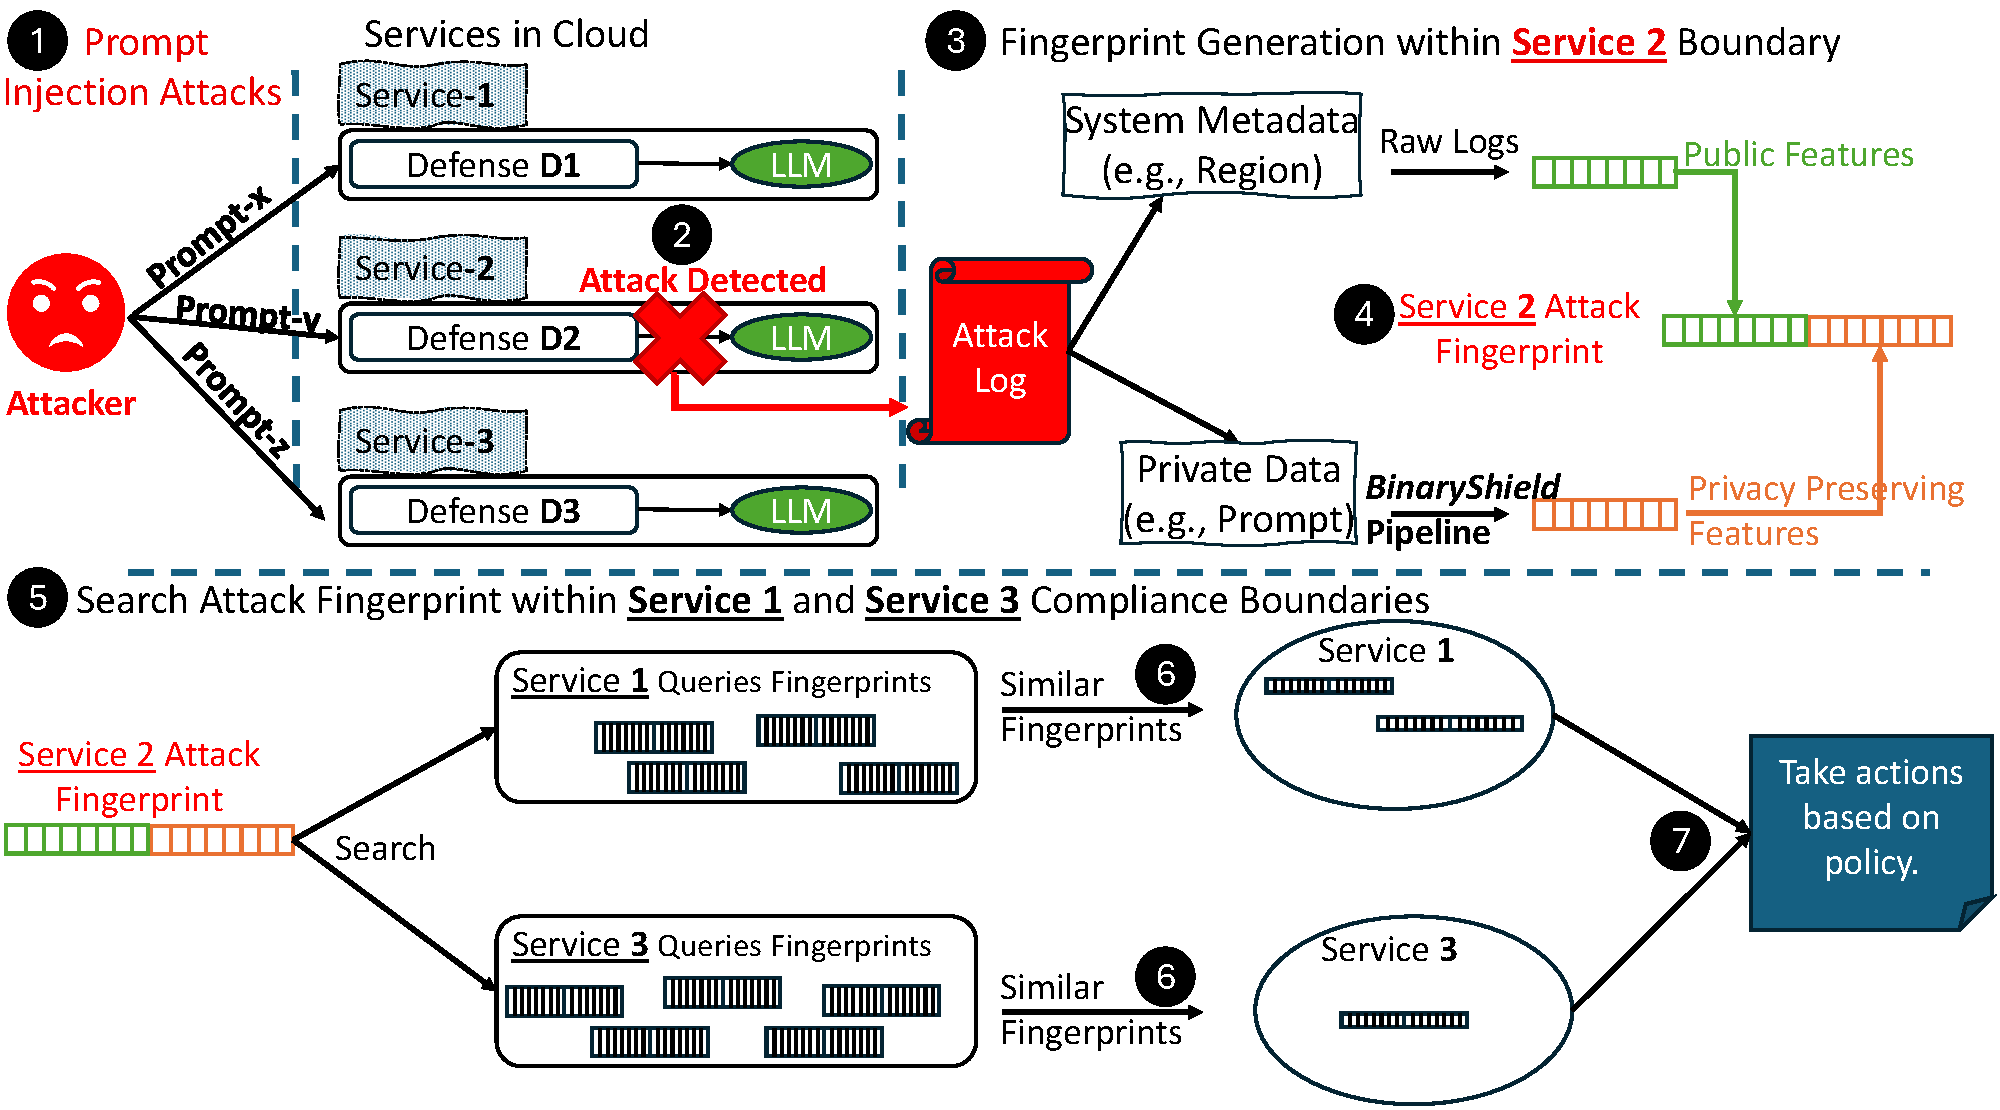
\includegraphics[width=0.95\linewidth]{sections/figures/BinaryShield-Architecture.pdf}
    \caption{\tool system design. Suspicious prompts are processed within the compliance boundary to generate privacy-preserving fingerprints, which are then shared across services for collaborative threat detection.}
    \label{fig:system-architecture}
    \vspace{-4mm}  
\end{figure}

\noindent\textbf{Evaluations.} We conduct comprehensive evaluation of \tool spanning threat correlation effectiveness, privacy calibration, scalability, and operational efficiency (Section~\ref{sec:evaluation}). 
\tool significantly outperforms privacy-preserving baseline across attack variants (17-point F1 advantage on sophisticated attacks) and exhibits smooth privacy-utility trade-offs with theoretical noise alignment. 
In real-world enterprise-scale scenarios, \tool achieves 79.2\% threat correlation accuracy (93\% of non-private baseline performance) alongside efficiency gains (38x search speedup).



